% Created by tikzDevice version 0.12.3 on 2020-02-05 13:44:44
% !TEX encoding = UTF-8 Unicode
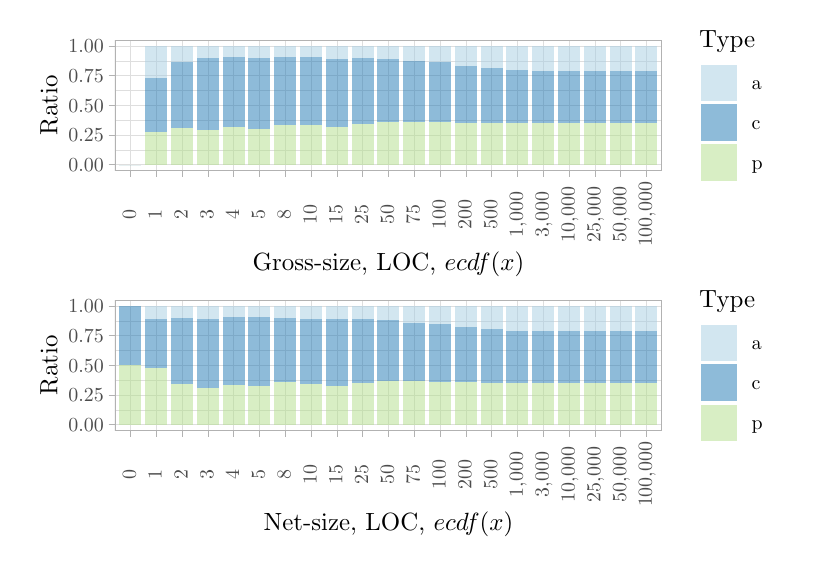
\begin{tikzpicture}[x=1pt,y=1pt]
\definecolor{fillColor}{RGB}{255,255,255}
\path[use as bounding box,fill=fillColor,fill opacity=0.00] (0,0) rectangle (274.63,187.90);
\begin{scope}
\path[clip] (  0.00, 93.95) rectangle (274.63,187.90);
\definecolor{drawColor}{RGB}{255,255,255}
\definecolor{fillColor}{RGB}{255,255,255}

\path[draw=drawColor,line width= 0.5pt,line join=round,line cap=round,fill=fillColor] (  0.00, 93.95) rectangle (274.63,187.90);
\end{scope}
\begin{scope}
\path[clip] ( 31.54,136.29) rectangle (229.17,183.40);
\definecolor{fillColor}{RGB}{255,255,255}

\path[fill=fillColor] ( 31.54,136.29) rectangle (229.17,183.40);
\definecolor{drawColor}{gray}{0.87}

\path[draw=drawColor,line width= 0.1pt,line join=round] ( 31.54,143.79) --
	(229.17,143.79);

\path[draw=drawColor,line width= 0.1pt,line join=round] ( 31.54,154.49) --
	(229.17,154.49);

\path[draw=drawColor,line width= 0.1pt,line join=round] ( 31.54,165.20) --
	(229.17,165.20);

\path[draw=drawColor,line width= 0.1pt,line join=round] ( 31.54,175.91) --
	(229.17,175.91);

\path[draw=drawColor,line width= 0.2pt,line join=round] ( 31.54,138.43) --
	(229.17,138.43);

\path[draw=drawColor,line width= 0.2pt,line join=round] ( 31.54,149.14) --
	(229.17,149.14);

\path[draw=drawColor,line width= 0.2pt,line join=round] ( 31.54,159.85) --
	(229.17,159.85);

\path[draw=drawColor,line width= 0.2pt,line join=round] ( 31.54,170.55) --
	(229.17,170.55);

\path[draw=drawColor,line width= 0.2pt,line join=round] ( 31.54,181.26) --
	(229.17,181.26);

\path[draw=drawColor,line width= 0.2pt,line join=round] ( 37.14,136.29) --
	( 37.14,183.40);

\path[draw=drawColor,line width= 0.2pt,line join=round] ( 46.46,136.29) --
	( 46.46,183.40);

\path[draw=drawColor,line width= 0.2pt,line join=round] ( 55.78,136.29) --
	( 55.78,183.40);

\path[draw=drawColor,line width= 0.2pt,line join=round] ( 65.10,136.29) --
	( 65.10,183.40);

\path[draw=drawColor,line width= 0.2pt,line join=round] ( 74.43,136.29) --
	( 74.43,183.40);

\path[draw=drawColor,line width= 0.2pt,line join=round] ( 83.75,136.29) --
	( 83.75,183.40);

\path[draw=drawColor,line width= 0.2pt,line join=round] ( 93.07,136.29) --
	( 93.07,183.40);

\path[draw=drawColor,line width= 0.2pt,line join=round] (102.39,136.29) --
	(102.39,183.40);

\path[draw=drawColor,line width= 0.2pt,line join=round] (111.71,136.29) --
	(111.71,183.40);

\path[draw=drawColor,line width= 0.2pt,line join=round] (121.04,136.29) --
	(121.04,183.40);

\path[draw=drawColor,line width= 0.2pt,line join=round] (130.36,136.29) --
	(130.36,183.40);

\path[draw=drawColor,line width= 0.2pt,line join=round] (139.68,136.29) --
	(139.68,183.40);

\path[draw=drawColor,line width= 0.2pt,line join=round] (149.00,136.29) --
	(149.00,183.40);

\path[draw=drawColor,line width= 0.2pt,line join=round] (158.33,136.29) --
	(158.33,183.40);

\path[draw=drawColor,line width= 0.2pt,line join=round] (167.65,136.29) --
	(167.65,183.40);

\path[draw=drawColor,line width= 0.2pt,line join=round] (176.97,136.29) --
	(176.97,183.40);

\path[draw=drawColor,line width= 0.2pt,line join=round] (186.29,136.29) --
	(186.29,183.40);

\path[draw=drawColor,line width= 0.2pt,line join=round] (195.61,136.29) --
	(195.61,183.40);

\path[draw=drawColor,line width= 0.2pt,line join=round] (204.94,136.29) --
	(204.94,183.40);

\path[draw=drawColor,line width= 0.2pt,line join=round] (214.26,136.29) --
	(214.26,183.40);

\path[draw=drawColor,line width= 0.2pt,line join=round] (223.58,136.29) --
	(223.58,183.40);
\definecolor{fillColor}{RGB}{178,223,138}

\path[fill=fillColor,fill opacity=0.50] ( 33.18,138.43) rectangle ( 41.10,138.43);
\definecolor{fillColor}{RGB}{31,120,180}

\path[fill=fillColor,fill opacity=0.50] ( 33.18,138.43) rectangle ( 41.10,138.43);
\definecolor{fillColor}{RGB}{166,206,227}

\path[fill=fillColor,fill opacity=0.50] ( 33.18,138.43) rectangle ( 41.10,138.43);
\definecolor{fillColor}{RGB}{178,223,138}

\path[fill=fillColor,fill opacity=0.50] ( 42.50,138.43) rectangle ( 50.42,150.11);
\definecolor{fillColor}{RGB}{31,120,180}

\path[fill=fillColor,fill opacity=0.50] ( 42.50,150.11) rectangle ( 50.42,169.58);
\definecolor{fillColor}{RGB}{166,206,227}

\path[fill=fillColor,fill opacity=0.50] ( 42.50,169.58) rectangle ( 50.42,181.26);
\definecolor{fillColor}{RGB}{178,223,138}

\path[fill=fillColor,fill opacity=0.50] ( 51.82,138.43) rectangle ( 59.74,151.47);
\definecolor{fillColor}{RGB}{31,120,180}

\path[fill=fillColor,fill opacity=0.50] ( 51.82,151.47) rectangle ( 59.74,175.67);
\definecolor{fillColor}{RGB}{166,206,227}

\path[fill=fillColor,fill opacity=0.50] ( 51.82,175.67) rectangle ( 59.74,181.26);
\definecolor{fillColor}{RGB}{178,223,138}

\path[fill=fillColor,fill opacity=0.50] ( 61.14,138.43) rectangle ( 69.07,151.09);
\definecolor{fillColor}{RGB}{31,120,180}

\path[fill=fillColor,fill opacity=0.50] ( 61.14,151.09) rectangle ( 69.07,176.88);
\definecolor{fillColor}{RGB}{166,206,227}

\path[fill=fillColor,fill opacity=0.50] ( 61.14,176.88) rectangle ( 69.07,181.26);
\definecolor{fillColor}{RGB}{178,223,138}

\path[fill=fillColor,fill opacity=0.50] ( 70.46,138.43) rectangle ( 78.39,151.94);
\definecolor{fillColor}{RGB}{31,120,180}

\path[fill=fillColor,fill opacity=0.50] ( 70.46,151.94) rectangle ( 78.39,177.31);
\definecolor{fillColor}{RGB}{166,206,227}

\path[fill=fillColor,fill opacity=0.50] ( 70.46,177.31) rectangle ( 78.39,181.26);
\definecolor{fillColor}{RGB}{178,223,138}

\path[fill=fillColor,fill opacity=0.50] ( 79.79,138.43) rectangle ( 87.71,151.40);
\definecolor{fillColor}{RGB}{31,120,180}

\path[fill=fillColor,fill opacity=0.50] ( 79.79,151.40) rectangle ( 87.71,177.03);
\definecolor{fillColor}{RGB}{166,206,227}

\path[fill=fillColor,fill opacity=0.50] ( 79.79,177.03) rectangle ( 87.71,181.26);
\definecolor{fillColor}{RGB}{178,223,138}

\path[fill=fillColor,fill opacity=0.50] ( 89.11,138.43) rectangle ( 97.03,152.65);
\definecolor{fillColor}{RGB}{31,120,180}

\path[fill=fillColor,fill opacity=0.50] ( 89.11,152.65) rectangle ( 97.03,177.37);
\definecolor{fillColor}{RGB}{166,206,227}

\path[fill=fillColor,fill opacity=0.50] ( 89.11,177.37) rectangle ( 97.03,181.26);
\definecolor{fillColor}{RGB}{178,223,138}

\path[fill=fillColor,fill opacity=0.50] ( 98.43,138.43) rectangle (106.35,152.71);
\definecolor{fillColor}{RGB}{31,120,180}

\path[fill=fillColor,fill opacity=0.50] ( 98.43,152.71) rectangle (106.35,177.32);
\definecolor{fillColor}{RGB}{166,206,227}

\path[fill=fillColor,fill opacity=0.50] ( 98.43,177.32) rectangle (106.35,181.26);
\definecolor{fillColor}{RGB}{178,223,138}

\path[fill=fillColor,fill opacity=0.50] (107.75,138.43) rectangle (115.68,151.87);
\definecolor{fillColor}{RGB}{31,120,180}

\path[fill=fillColor,fill opacity=0.50] (107.75,151.87) rectangle (115.68,176.61);
\definecolor{fillColor}{RGB}{166,206,227}

\path[fill=fillColor,fill opacity=0.50] (107.75,176.61) rectangle (115.68,181.26);
\definecolor{fillColor}{RGB}{178,223,138}

\path[fill=fillColor,fill opacity=0.50] (117.07,138.43) rectangle (125.00,153.07);
\definecolor{fillColor}{RGB}{31,120,180}

\path[fill=fillColor,fill opacity=0.50] (117.07,153.07) rectangle (125.00,177.00);
\definecolor{fillColor}{RGB}{166,206,227}

\path[fill=fillColor,fill opacity=0.50] (117.07,177.00) rectangle (125.00,181.26);
\definecolor{fillColor}{RGB}{178,223,138}

\path[fill=fillColor,fill opacity=0.50] (126.40,138.43) rectangle (134.32,153.75);
\definecolor{fillColor}{RGB}{31,120,180}

\path[fill=fillColor,fill opacity=0.50] (126.40,153.75) rectangle (134.32,176.72);
\definecolor{fillColor}{RGB}{166,206,227}

\path[fill=fillColor,fill opacity=0.50] (126.40,176.72) rectangle (134.32,181.26);
\definecolor{fillColor}{RGB}{178,223,138}

\path[fill=fillColor,fill opacity=0.50] (135.72,138.43) rectangle (143.64,153.79);
\definecolor{fillColor}{RGB}{31,120,180}

\path[fill=fillColor,fill opacity=0.50] (135.72,153.79) rectangle (143.64,175.90);
\definecolor{fillColor}{RGB}{166,206,227}

\path[fill=fillColor,fill opacity=0.50] (135.72,175.90) rectangle (143.64,181.26);
\definecolor{fillColor}{RGB}{178,223,138}

\path[fill=fillColor,fill opacity=0.50] (145.04,138.43) rectangle (152.96,153.87);
\definecolor{fillColor}{RGB}{31,120,180}

\path[fill=fillColor,fill opacity=0.50] (145.04,153.87) rectangle (152.96,175.53);
\definecolor{fillColor}{RGB}{166,206,227}

\path[fill=fillColor,fill opacity=0.50] (145.04,175.53) rectangle (152.96,181.26);
\definecolor{fillColor}{RGB}{178,223,138}

\path[fill=fillColor,fill opacity=0.50] (154.36,138.43) rectangle (162.29,153.59);
\definecolor{fillColor}{RGB}{31,120,180}

\path[fill=fillColor,fill opacity=0.50] (154.36,153.59) rectangle (162.29,174.10);
\definecolor{fillColor}{RGB}{166,206,227}

\path[fill=fillColor,fill opacity=0.50] (154.36,174.10) rectangle (162.29,181.26);
\definecolor{fillColor}{RGB}{178,223,138}

\path[fill=fillColor,fill opacity=0.50] (163.69,138.43) rectangle (171.61,153.63);
\definecolor{fillColor}{RGB}{31,120,180}

\path[fill=fillColor,fill opacity=0.50] (163.69,153.63) rectangle (171.61,173.16);
\definecolor{fillColor}{RGB}{166,206,227}

\path[fill=fillColor,fill opacity=0.50] (163.69,173.16) rectangle (171.61,181.26);
\definecolor{fillColor}{RGB}{178,223,138}

\path[fill=fillColor,fill opacity=0.50] (173.01,138.43) rectangle (180.93,153.52);
\definecolor{fillColor}{RGB}{31,120,180}

\path[fill=fillColor,fill opacity=0.50] (173.01,153.52) rectangle (180.93,172.57);
\definecolor{fillColor}{RGB}{166,206,227}

\path[fill=fillColor,fill opacity=0.50] (173.01,172.57) rectangle (180.93,181.26);
\definecolor{fillColor}{RGB}{178,223,138}

\path[fill=fillColor,fill opacity=0.50] (182.33,138.43) rectangle (190.25,153.46);
\definecolor{fillColor}{RGB}{31,120,180}

\path[fill=fillColor,fill opacity=0.50] (182.33,153.46) rectangle (190.25,172.22);
\definecolor{fillColor}{RGB}{166,206,227}

\path[fill=fillColor,fill opacity=0.50] (182.33,172.22) rectangle (190.25,181.26);
\definecolor{fillColor}{RGB}{178,223,138}

\path[fill=fillColor,fill opacity=0.50] (191.65,138.43) rectangle (199.58,153.44);
\definecolor{fillColor}{RGB}{31,120,180}

\path[fill=fillColor,fill opacity=0.50] (191.65,153.44) rectangle (199.58,172.08);
\definecolor{fillColor}{RGB}{166,206,227}

\path[fill=fillColor,fill opacity=0.50] (191.65,172.08) rectangle (199.58,181.26);
\definecolor{fillColor}{RGB}{178,223,138}

\path[fill=fillColor,fill opacity=0.50] (200.97,138.43) rectangle (208.90,153.46);
\definecolor{fillColor}{RGB}{31,120,180}

\path[fill=fillColor,fill opacity=0.50] (200.97,153.46) rectangle (208.90,172.09);
\definecolor{fillColor}{RGB}{166,206,227}

\path[fill=fillColor,fill opacity=0.50] (200.97,172.09) rectangle (208.90,181.26);
\definecolor{fillColor}{RGB}{178,223,138}

\path[fill=fillColor,fill opacity=0.50] (210.30,138.43) rectangle (218.22,153.46);
\definecolor{fillColor}{RGB}{31,120,180}

\path[fill=fillColor,fill opacity=0.50] (210.30,153.46) rectangle (218.22,172.09);
\definecolor{fillColor}{RGB}{166,206,227}

\path[fill=fillColor,fill opacity=0.50] (210.30,172.09) rectangle (218.22,181.26);
\definecolor{fillColor}{RGB}{178,223,138}

\path[fill=fillColor,fill opacity=0.50] (219.62,138.43) rectangle (227.54,153.46);
\definecolor{fillColor}{RGB}{31,120,180}

\path[fill=fillColor,fill opacity=0.50] (219.62,153.46) rectangle (227.54,172.09);
\definecolor{fillColor}{RGB}{166,206,227}

\path[fill=fillColor,fill opacity=0.50] (219.62,172.09) rectangle (227.54,181.26);
\definecolor{drawColor}{gray}{0.70}

\path[draw=drawColor,line width= 0.5pt,line join=round,line cap=round] ( 31.54,136.29) rectangle (229.17,183.40);
\end{scope}
\begin{scope}
\path[clip] (  0.00,  0.00) rectangle (274.63,187.90);
\definecolor{drawColor}{gray}{0.30}

\node[text=drawColor,anchor=base east,inner sep=0pt, outer sep=0pt, scale=  0.72] at ( 27.49,135.96) {0.00};

\node[text=drawColor,anchor=base east,inner sep=0pt, outer sep=0pt, scale=  0.72] at ( 27.49,146.66) {0.25};

\node[text=drawColor,anchor=base east,inner sep=0pt, outer sep=0pt, scale=  0.72] at ( 27.49,157.37) {0.50};

\node[text=drawColor,anchor=base east,inner sep=0pt, outer sep=0pt, scale=  0.72] at ( 27.49,168.07) {0.75};

\node[text=drawColor,anchor=base east,inner sep=0pt, outer sep=0pt, scale=  0.72] at ( 27.49,178.78) {1.00};
\end{scope}
\begin{scope}
\path[clip] (  0.00,  0.00) rectangle (274.63,187.90);
\definecolor{drawColor}{gray}{0.70}

\path[draw=drawColor,line width= 0.2pt,line join=round] ( 29.29,138.43) --
	( 31.54,138.43);

\path[draw=drawColor,line width= 0.2pt,line join=round] ( 29.29,149.14) --
	( 31.54,149.14);

\path[draw=drawColor,line width= 0.2pt,line join=round] ( 29.29,159.85) --
	( 31.54,159.85);

\path[draw=drawColor,line width= 0.2pt,line join=round] ( 29.29,170.55) --
	( 31.54,170.55);

\path[draw=drawColor,line width= 0.2pt,line join=round] ( 29.29,181.26) --
	( 31.54,181.26);
\end{scope}
\begin{scope}
\path[clip] (  0.00,  0.00) rectangle (274.63,187.90);
\definecolor{drawColor}{gray}{0.70}

\path[draw=drawColor,line width= 0.2pt,line join=round] ( 37.14,134.04) --
	( 37.14,136.29);

\path[draw=drawColor,line width= 0.2pt,line join=round] ( 46.46,134.04) --
	( 46.46,136.29);

\path[draw=drawColor,line width= 0.2pt,line join=round] ( 55.78,134.04) --
	( 55.78,136.29);

\path[draw=drawColor,line width= 0.2pt,line join=round] ( 65.10,134.04) --
	( 65.10,136.29);

\path[draw=drawColor,line width= 0.2pt,line join=round] ( 74.43,134.04) --
	( 74.43,136.29);

\path[draw=drawColor,line width= 0.2pt,line join=round] ( 83.75,134.04) --
	( 83.75,136.29);

\path[draw=drawColor,line width= 0.2pt,line join=round] ( 93.07,134.04) --
	( 93.07,136.29);

\path[draw=drawColor,line width= 0.2pt,line join=round] (102.39,134.04) --
	(102.39,136.29);

\path[draw=drawColor,line width= 0.2pt,line join=round] (111.71,134.04) --
	(111.71,136.29);

\path[draw=drawColor,line width= 0.2pt,line join=round] (121.04,134.04) --
	(121.04,136.29);

\path[draw=drawColor,line width= 0.2pt,line join=round] (130.36,134.04) --
	(130.36,136.29);

\path[draw=drawColor,line width= 0.2pt,line join=round] (139.68,134.04) --
	(139.68,136.29);

\path[draw=drawColor,line width= 0.2pt,line join=round] (149.00,134.04) --
	(149.00,136.29);

\path[draw=drawColor,line width= 0.2pt,line join=round] (158.33,134.04) --
	(158.33,136.29);

\path[draw=drawColor,line width= 0.2pt,line join=round] (167.65,134.04) --
	(167.65,136.29);

\path[draw=drawColor,line width= 0.2pt,line join=round] (176.97,134.04) --
	(176.97,136.29);

\path[draw=drawColor,line width= 0.2pt,line join=round] (186.29,134.04) --
	(186.29,136.29);

\path[draw=drawColor,line width= 0.2pt,line join=round] (195.61,134.04) --
	(195.61,136.29);

\path[draw=drawColor,line width= 0.2pt,line join=round] (204.94,134.04) --
	(204.94,136.29);

\path[draw=drawColor,line width= 0.2pt,line join=round] (214.26,134.04) --
	(214.26,136.29);

\path[draw=drawColor,line width= 0.2pt,line join=round] (223.58,134.04) --
	(223.58,136.29);
\end{scope}
\begin{scope}
\path[clip] (  0.00,  0.00) rectangle (274.63,187.90);
\definecolor{drawColor}{gray}{0.30}

\node[text=drawColor,rotate= 90.00,anchor=base,inner sep=0pt, outer sep=0pt, scale=  0.72] at ( 39.12,120.45) {      0};

\node[text=drawColor,rotate= 90.00,anchor=base,inner sep=0pt, outer sep=0pt, scale=  0.72] at ( 48.44,120.45) {      1};

\node[text=drawColor,rotate= 90.00,anchor=base,inner sep=0pt, outer sep=0pt, scale=  0.72] at ( 57.77,120.45) {      2};

\node[text=drawColor,rotate= 90.00,anchor=base,inner sep=0pt, outer sep=0pt, scale=  0.72] at ( 67.09,120.45) {      3};

\node[text=drawColor,rotate= 90.00,anchor=base,inner sep=0pt, outer sep=0pt, scale=  0.72] at ( 76.41,120.45) {      4};

\node[text=drawColor,rotate= 90.00,anchor=base,inner sep=0pt, outer sep=0pt, scale=  0.72] at ( 85.73,120.45) {      5};

\node[text=drawColor,rotate= 90.00,anchor=base,inner sep=0pt, outer sep=0pt, scale=  0.72] at ( 95.05,120.45) {      8};

\node[text=drawColor,rotate= 90.00,anchor=base,inner sep=0pt, outer sep=0pt, scale=  0.72] at (104.38,120.45) {     10};

\node[text=drawColor,rotate= 90.00,anchor=base,inner sep=0pt, outer sep=0pt, scale=  0.72] at (113.70,120.45) {     15};

\node[text=drawColor,rotate= 90.00,anchor=base,inner sep=0pt, outer sep=0pt, scale=  0.72] at (123.02,120.45) {     25};

\node[text=drawColor,rotate= 90.00,anchor=base,inner sep=0pt, outer sep=0pt, scale=  0.72] at (132.34,120.45) {     50};

\node[text=drawColor,rotate= 90.00,anchor=base,inner sep=0pt, outer sep=0pt, scale=  0.72] at (141.66,120.45) {     75};

\node[text=drawColor,rotate= 90.00,anchor=base,inner sep=0pt, outer sep=0pt, scale=  0.72] at (150.99,120.45) {    100};

\node[text=drawColor,rotate= 90.00,anchor=base,inner sep=0pt, outer sep=0pt, scale=  0.72] at (160.31,120.45) {    200};

\node[text=drawColor,rotate= 90.00,anchor=base,inner sep=0pt, outer sep=0pt, scale=  0.72] at (169.63,120.45) {    500};

\node[text=drawColor,rotate= 90.00,anchor=base,inner sep=0pt, outer sep=0pt, scale=  0.72] at (178.95,120.45) {  1,000};

\node[text=drawColor,rotate= 90.00,anchor=base,inner sep=0pt, outer sep=0pt, scale=  0.72] at (188.27,120.45) {  3,000};

\node[text=drawColor,rotate= 90.00,anchor=base,inner sep=0pt, outer sep=0pt, scale=  0.72] at (197.60,120.45) { 10,000};

\node[text=drawColor,rotate= 90.00,anchor=base,inner sep=0pt, outer sep=0pt, scale=  0.72] at (206.92,120.45) { 25,000};

\node[text=drawColor,rotate= 90.00,anchor=base,inner sep=0pt, outer sep=0pt, scale=  0.72] at (216.24,120.45) { 50,000};

\node[text=drawColor,rotate= 90.00,anchor=base,inner sep=0pt, outer sep=0pt, scale=  0.72] at (225.56,120.45) {100,000};
\end{scope}
\begin{scope}
\path[clip] (  0.00,  0.00) rectangle (274.63,187.90);
\definecolor{drawColor}{RGB}{0,0,0}

\node[text=drawColor,anchor=base,inner sep=0pt, outer sep=0pt, scale=  0.90] at (130.36,100.20) {Gross-size, LOC, $ecdf(x)$};
\end{scope}
\begin{scope}
\path[clip] (  0.00,  0.00) rectangle (274.63,187.90);
\definecolor{drawColor}{RGB}{0,0,0}

\node[text=drawColor,rotate= 90.00,anchor=base,inner sep=0pt, outer sep=0pt, scale=  0.90] at ( 10.70,159.85) {Ratio};
\end{scope}
\begin{scope}
\path[clip] (  0.00,  0.00) rectangle (274.63,187.90);
\definecolor{fillColor}{RGB}{255,255,255}

\path[fill=fillColor] (238.17,127.44) rectangle (270.13,192.25);
\end{scope}
\begin{scope}
\path[clip] (  0.00,  0.00) rectangle (274.63,187.90);
\definecolor{drawColor}{RGB}{0,0,0}

\node[text=drawColor,anchor=base west,inner sep=0pt, outer sep=0pt, scale=  0.90] at (242.67,180.68) {Type};
\end{scope}
\begin{scope}
\path[clip] (  0.00,  0.00) rectangle (274.63,187.90);
\definecolor{fillColor}{RGB}{255,255,255}

\path[fill=fillColor] (242.67,160.85) rectangle (257.13,175.30);
\end{scope}
\begin{scope}
\path[clip] (  0.00,  0.00) rectangle (274.63,187.90);
\definecolor{fillColor}{RGB}{166,206,227}

\path[fill=fillColor,fill opacity=0.50] (243.38,161.56) rectangle (256.42,174.59);
\end{scope}
\begin{scope}
\path[clip] (  0.00,  0.00) rectangle (274.63,187.90);
\definecolor{fillColor}{RGB}{255,255,255}

\path[fill=fillColor] (242.67,146.40) rectangle (257.13,160.85);
\end{scope}
\begin{scope}
\path[clip] (  0.00,  0.00) rectangle (274.63,187.90);
\definecolor{fillColor}{RGB}{31,120,180}

\path[fill=fillColor,fill opacity=0.50] (243.38,147.11) rectangle (256.42,160.14);
\end{scope}
\begin{scope}
\path[clip] (  0.00,  0.00) rectangle (274.63,187.90);
\definecolor{fillColor}{RGB}{255,255,255}

\path[fill=fillColor] (242.67,131.94) rectangle (257.13,146.40);
\end{scope}
\begin{scope}
\path[clip] (  0.00,  0.00) rectangle (274.63,187.90);
\definecolor{fillColor}{RGB}{178,223,138}

\path[fill=fillColor,fill opacity=0.50] (243.38,132.65) rectangle (256.42,145.69);
\end{scope}
\begin{scope}
\path[clip] (  0.00,  0.00) rectangle (274.63,187.90);
\definecolor{drawColor}{RGB}{0,0,0}

\node[text=drawColor,anchor=base west,inner sep=0pt, outer sep=0pt, scale=  0.72] at (261.63,165.60) {a};
\end{scope}
\begin{scope}
\path[clip] (  0.00,  0.00) rectangle (274.63,187.90);
\definecolor{drawColor}{RGB}{0,0,0}

\node[text=drawColor,anchor=base west,inner sep=0pt, outer sep=0pt, scale=  0.72] at (261.63,151.14) {c};
\end{scope}
\begin{scope}
\path[clip] (  0.00,  0.00) rectangle (274.63,187.90);
\definecolor{drawColor}{RGB}{0,0,0}

\node[text=drawColor,anchor=base west,inner sep=0pt, outer sep=0pt, scale=  0.72] at (261.63,136.69) {p};
\end{scope}
\begin{scope}
\path[clip] (  0.00,  0.00) rectangle (274.63, 93.95);
\definecolor{drawColor}{RGB}{255,255,255}
\definecolor{fillColor}{RGB}{255,255,255}

\path[draw=drawColor,line width= 0.5pt,line join=round,line cap=round,fill=fillColor] (  0.00,  0.00) rectangle (274.63, 93.95);
\end{scope}
\begin{scope}
\path[clip] ( 31.54, 42.34) rectangle (229.17, 89.45);
\definecolor{fillColor}{RGB}{255,255,255}

\path[fill=fillColor] ( 31.54, 42.34) rectangle (229.17, 89.45);
\definecolor{drawColor}{gray}{0.87}

\path[draw=drawColor,line width= 0.1pt,line join=round] ( 31.54, 49.84) --
	(229.17, 49.84);

\path[draw=drawColor,line width= 0.1pt,line join=round] ( 31.54, 60.54) --
	(229.17, 60.54);

\path[draw=drawColor,line width= 0.1pt,line join=round] ( 31.54, 71.25) --
	(229.17, 71.25);

\path[draw=drawColor,line width= 0.1pt,line join=round] ( 31.54, 81.96) --
	(229.17, 81.96);

\path[draw=drawColor,line width= 0.2pt,line join=round] ( 31.54, 44.48) --
	(229.17, 44.48);

\path[draw=drawColor,line width= 0.2pt,line join=round] ( 31.54, 55.19) --
	(229.17, 55.19);

\path[draw=drawColor,line width= 0.2pt,line join=round] ( 31.54, 65.90) --
	(229.17, 65.90);

\path[draw=drawColor,line width= 0.2pt,line join=round] ( 31.54, 76.60) --
	(229.17, 76.60);

\path[draw=drawColor,line width= 0.2pt,line join=round] ( 31.54, 87.31) --
	(229.17, 87.31);

\path[draw=drawColor,line width= 0.2pt,line join=round] ( 37.14, 42.34) --
	( 37.14, 89.45);

\path[draw=drawColor,line width= 0.2pt,line join=round] ( 46.46, 42.34) --
	( 46.46, 89.45);

\path[draw=drawColor,line width= 0.2pt,line join=round] ( 55.78, 42.34) --
	( 55.78, 89.45);

\path[draw=drawColor,line width= 0.2pt,line join=round] ( 65.10, 42.34) --
	( 65.10, 89.45);

\path[draw=drawColor,line width= 0.2pt,line join=round] ( 74.43, 42.34) --
	( 74.43, 89.45);

\path[draw=drawColor,line width= 0.2pt,line join=round] ( 83.75, 42.34) --
	( 83.75, 89.45);

\path[draw=drawColor,line width= 0.2pt,line join=round] ( 93.07, 42.34) --
	( 93.07, 89.45);

\path[draw=drawColor,line width= 0.2pt,line join=round] (102.39, 42.34) --
	(102.39, 89.45);

\path[draw=drawColor,line width= 0.2pt,line join=round] (111.71, 42.34) --
	(111.71, 89.45);

\path[draw=drawColor,line width= 0.2pt,line join=round] (121.04, 42.34) --
	(121.04, 89.45);

\path[draw=drawColor,line width= 0.2pt,line join=round] (130.36, 42.34) --
	(130.36, 89.45);

\path[draw=drawColor,line width= 0.2pt,line join=round] (139.68, 42.34) --
	(139.68, 89.45);

\path[draw=drawColor,line width= 0.2pt,line join=round] (149.00, 42.34) --
	(149.00, 89.45);

\path[draw=drawColor,line width= 0.2pt,line join=round] (158.33, 42.34) --
	(158.33, 89.45);

\path[draw=drawColor,line width= 0.2pt,line join=round] (167.65, 42.34) --
	(167.65, 89.45);

\path[draw=drawColor,line width= 0.2pt,line join=round] (176.97, 42.34) --
	(176.97, 89.45);

\path[draw=drawColor,line width= 0.2pt,line join=round] (186.29, 42.34) --
	(186.29, 89.45);

\path[draw=drawColor,line width= 0.2pt,line join=round] (195.61, 42.34) --
	(195.61, 89.45);

\path[draw=drawColor,line width= 0.2pt,line join=round] (204.94, 42.34) --
	(204.94, 89.45);

\path[draw=drawColor,line width= 0.2pt,line join=round] (214.26, 42.34) --
	(214.26, 89.45);

\path[draw=drawColor,line width= 0.2pt,line join=round] (223.58, 42.34) --
	(223.58, 89.45);
\definecolor{fillColor}{RGB}{178,223,138}

\path[fill=fillColor,fill opacity=0.50] ( 33.18, 44.48) rectangle ( 41.10, 65.90);
\definecolor{fillColor}{RGB}{31,120,180}

\path[fill=fillColor,fill opacity=0.50] ( 33.18, 65.90) rectangle ( 41.10, 87.31);
\definecolor{fillColor}{RGB}{166,206,227}

\path[fill=fillColor,fill opacity=0.50] ( 33.18, 87.31) rectangle ( 41.10, 87.31);
\definecolor{fillColor}{RGB}{178,223,138}

\path[fill=fillColor,fill opacity=0.50] ( 42.50, 44.48) rectangle ( 50.42, 65.10);
\definecolor{fillColor}{RGB}{31,120,180}

\path[fill=fillColor,fill opacity=0.50] ( 42.50, 65.10) rectangle ( 50.42, 82.55);
\definecolor{fillColor}{RGB}{166,206,227}

\path[fill=fillColor,fill opacity=0.50] ( 42.50, 82.55) rectangle ( 50.42, 87.31);
\definecolor{fillColor}{RGB}{178,223,138}

\path[fill=fillColor,fill opacity=0.50] ( 51.82, 44.48) rectangle ( 59.74, 59.23);
\definecolor{fillColor}{RGB}{31,120,180}

\path[fill=fillColor,fill opacity=0.50] ( 51.82, 59.23) rectangle ( 59.74, 83.03);
\definecolor{fillColor}{RGB}{166,206,227}

\path[fill=fillColor,fill opacity=0.50] ( 51.82, 83.03) rectangle ( 59.74, 87.31);
\definecolor{fillColor}{RGB}{178,223,138}

\path[fill=fillColor,fill opacity=0.50] ( 61.14, 44.48) rectangle ( 69.07, 57.55);
\definecolor{fillColor}{RGB}{31,120,180}

\path[fill=fillColor,fill opacity=0.50] ( 61.14, 57.55) rectangle ( 69.07, 82.59);
\definecolor{fillColor}{RGB}{166,206,227}

\path[fill=fillColor,fill opacity=0.50] ( 61.14, 82.59) rectangle ( 69.07, 87.31);
\definecolor{fillColor}{RGB}{178,223,138}

\path[fill=fillColor,fill opacity=0.50] ( 70.46, 44.48) rectangle ( 78.39, 58.76);
\definecolor{fillColor}{RGB}{31,120,180}

\path[fill=fillColor,fill opacity=0.50] ( 70.46, 58.76) rectangle ( 78.39, 83.34);
\definecolor{fillColor}{RGB}{166,206,227}

\path[fill=fillColor,fill opacity=0.50] ( 70.46, 83.34) rectangle ( 78.39, 87.31);
\definecolor{fillColor}{RGB}{178,223,138}

\path[fill=fillColor,fill opacity=0.50] ( 79.79, 44.48) rectangle ( 87.71, 58.52);
\definecolor{fillColor}{RGB}{31,120,180}

\path[fill=fillColor,fill opacity=0.50] ( 79.79, 58.52) rectangle ( 87.71, 83.50);
\definecolor{fillColor}{RGB}{166,206,227}

\path[fill=fillColor,fill opacity=0.50] ( 79.79, 83.50) rectangle ( 87.71, 87.31);
\definecolor{fillColor}{RGB}{178,223,138}

\path[fill=fillColor,fill opacity=0.50] ( 89.11, 44.48) rectangle ( 97.03, 59.77);
\definecolor{fillColor}{RGB}{31,120,180}

\path[fill=fillColor,fill opacity=0.50] ( 89.11, 59.77) rectangle ( 97.03, 83.11);
\definecolor{fillColor}{RGB}{166,206,227}

\path[fill=fillColor,fill opacity=0.50] ( 89.11, 83.11) rectangle ( 97.03, 87.31);
\definecolor{fillColor}{RGB}{178,223,138}

\path[fill=fillColor,fill opacity=0.50] ( 98.43, 44.48) rectangle (106.35, 59.13);
\definecolor{fillColor}{RGB}{31,120,180}

\path[fill=fillColor,fill opacity=0.50] ( 98.43, 59.13) rectangle (106.35, 82.80);
\definecolor{fillColor}{RGB}{166,206,227}

\path[fill=fillColor,fill opacity=0.50] ( 98.43, 82.80) rectangle (106.35, 87.31);
\definecolor{fillColor}{RGB}{178,223,138}

\path[fill=fillColor,fill opacity=0.50] (107.75, 44.48) rectangle (115.68, 58.57);
\definecolor{fillColor}{RGB}{31,120,180}

\path[fill=fillColor,fill opacity=0.50] (107.75, 58.57) rectangle (115.68, 82.54);
\definecolor{fillColor}{RGB}{166,206,227}

\path[fill=fillColor,fill opacity=0.50] (107.75, 82.54) rectangle (115.68, 87.31);
\definecolor{fillColor}{RGB}{178,223,138}

\path[fill=fillColor,fill opacity=0.50] (117.07, 44.48) rectangle (125.00, 59.38);
\definecolor{fillColor}{RGB}{31,120,180}

\path[fill=fillColor,fill opacity=0.50] (117.07, 59.38) rectangle (125.00, 82.74);
\definecolor{fillColor}{RGB}{166,206,227}

\path[fill=fillColor,fill opacity=0.50] (117.07, 82.74) rectangle (125.00, 87.31);
\definecolor{fillColor}{RGB}{178,223,138}

\path[fill=fillColor,fill opacity=0.50] (126.40, 44.48) rectangle (134.32, 60.10);
\definecolor{fillColor}{RGB}{31,120,180}

\path[fill=fillColor,fill opacity=0.50] (126.40, 60.10) rectangle (134.32, 82.25);
\definecolor{fillColor}{RGB}{166,206,227}

\path[fill=fillColor,fill opacity=0.50] (126.40, 82.25) rectangle (134.32, 87.31);
\definecolor{fillColor}{RGB}{178,223,138}

\path[fill=fillColor,fill opacity=0.50] (135.72, 44.48) rectangle (143.64, 60.13);
\definecolor{fillColor}{RGB}{31,120,180}

\path[fill=fillColor,fill opacity=0.50] (135.72, 60.13) rectangle (143.64, 81.33);
\definecolor{fillColor}{RGB}{166,206,227}

\path[fill=fillColor,fill opacity=0.50] (135.72, 81.33) rectangle (143.64, 87.31);
\definecolor{fillColor}{RGB}{178,223,138}

\path[fill=fillColor,fill opacity=0.50] (145.04, 44.48) rectangle (152.96, 59.98);
\definecolor{fillColor}{RGB}{31,120,180}

\path[fill=fillColor,fill opacity=0.50] (145.04, 59.98) rectangle (152.96, 80.78);
\definecolor{fillColor}{RGB}{166,206,227}

\path[fill=fillColor,fill opacity=0.50] (145.04, 80.78) rectangle (152.96, 87.31);
\definecolor{fillColor}{RGB}{178,223,138}

\path[fill=fillColor,fill opacity=0.50] (154.36, 44.48) rectangle (162.29, 59.92);
\definecolor{fillColor}{RGB}{31,120,180}

\path[fill=fillColor,fill opacity=0.50] (154.36, 59.92) rectangle (162.29, 79.66);
\definecolor{fillColor}{RGB}{166,206,227}

\path[fill=fillColor,fill opacity=0.50] (154.36, 79.66) rectangle (162.29, 87.31);
\definecolor{fillColor}{RGB}{178,223,138}

\path[fill=fillColor,fill opacity=0.50] (163.69, 44.48) rectangle (171.61, 59.58);
\definecolor{fillColor}{RGB}{31,120,180}

\path[fill=fillColor,fill opacity=0.50] (163.69, 59.58) rectangle (171.61, 78.87);
\definecolor{fillColor}{RGB}{166,206,227}

\path[fill=fillColor,fill opacity=0.50] (163.69, 78.87) rectangle (171.61, 87.31);
\definecolor{fillColor}{RGB}{178,223,138}

\path[fill=fillColor,fill opacity=0.50] (173.01, 44.48) rectangle (180.93, 59.60);
\definecolor{fillColor}{RGB}{31,120,180}

\path[fill=fillColor,fill opacity=0.50] (173.01, 59.60) rectangle (180.93, 78.47);
\definecolor{fillColor}{RGB}{166,206,227}

\path[fill=fillColor,fill opacity=0.50] (173.01, 78.47) rectangle (180.93, 87.31);
\definecolor{fillColor}{RGB}{178,223,138}

\path[fill=fillColor,fill opacity=0.50] (182.33, 44.48) rectangle (190.25, 59.53);
\definecolor{fillColor}{RGB}{31,120,180}

\path[fill=fillColor,fill opacity=0.50] (182.33, 59.53) rectangle (190.25, 78.18);
\definecolor{fillColor}{RGB}{166,206,227}

\path[fill=fillColor,fill opacity=0.50] (182.33, 78.18) rectangle (190.25, 87.31);
\definecolor{fillColor}{RGB}{178,223,138}

\path[fill=fillColor,fill opacity=0.50] (191.65, 44.48) rectangle (199.58, 59.48);
\definecolor{fillColor}{RGB}{31,120,180}

\path[fill=fillColor,fill opacity=0.50] (191.65, 59.48) rectangle (199.58, 78.13);
\definecolor{fillColor}{RGB}{166,206,227}

\path[fill=fillColor,fill opacity=0.50] (191.65, 78.13) rectangle (199.58, 87.31);
\definecolor{fillColor}{RGB}{178,223,138}

\path[fill=fillColor,fill opacity=0.50] (200.97, 44.48) rectangle (208.90, 59.50);
\definecolor{fillColor}{RGB}{31,120,180}

\path[fill=fillColor,fill opacity=0.50] (200.97, 59.50) rectangle (208.90, 78.14);
\definecolor{fillColor}{RGB}{166,206,227}

\path[fill=fillColor,fill opacity=0.50] (200.97, 78.14) rectangle (208.90, 87.31);
\definecolor{fillColor}{RGB}{178,223,138}

\path[fill=fillColor,fill opacity=0.50] (210.30, 44.48) rectangle (218.22, 59.50);
\definecolor{fillColor}{RGB}{31,120,180}

\path[fill=fillColor,fill opacity=0.50] (210.30, 59.50) rectangle (218.22, 78.14);
\definecolor{fillColor}{RGB}{166,206,227}

\path[fill=fillColor,fill opacity=0.50] (210.30, 78.14) rectangle (218.22, 87.31);
\definecolor{fillColor}{RGB}{178,223,138}

\path[fill=fillColor,fill opacity=0.50] (219.62, 44.48) rectangle (227.54, 59.50);
\definecolor{fillColor}{RGB}{31,120,180}

\path[fill=fillColor,fill opacity=0.50] (219.62, 59.50) rectangle (227.54, 78.14);
\definecolor{fillColor}{RGB}{166,206,227}

\path[fill=fillColor,fill opacity=0.50] (219.62, 78.14) rectangle (227.54, 87.31);
\definecolor{drawColor}{gray}{0.70}

\path[draw=drawColor,line width= 0.5pt,line join=round,line cap=round] ( 31.54, 42.34) rectangle (229.17, 89.45);
\end{scope}
\begin{scope}
\path[clip] (  0.00,  0.00) rectangle (274.63,187.90);
\definecolor{drawColor}{gray}{0.30}

\node[text=drawColor,anchor=base east,inner sep=0pt, outer sep=0pt, scale=  0.72] at ( 27.49, 42.00) {0.00};

\node[text=drawColor,anchor=base east,inner sep=0pt, outer sep=0pt, scale=  0.72] at ( 27.49, 52.71) {0.25};

\node[text=drawColor,anchor=base east,inner sep=0pt, outer sep=0pt, scale=  0.72] at ( 27.49, 63.42) {0.50};

\node[text=drawColor,anchor=base east,inner sep=0pt, outer sep=0pt, scale=  0.72] at ( 27.49, 74.12) {0.75};

\node[text=drawColor,anchor=base east,inner sep=0pt, outer sep=0pt, scale=  0.72] at ( 27.49, 84.83) {1.00};
\end{scope}
\begin{scope}
\path[clip] (  0.00,  0.00) rectangle (274.63,187.90);
\definecolor{drawColor}{gray}{0.70}

\path[draw=drawColor,line width= 0.2pt,line join=round] ( 29.29, 44.48) --
	( 31.54, 44.48);

\path[draw=drawColor,line width= 0.2pt,line join=round] ( 29.29, 55.19) --
	( 31.54, 55.19);

\path[draw=drawColor,line width= 0.2pt,line join=round] ( 29.29, 65.90) --
	( 31.54, 65.90);

\path[draw=drawColor,line width= 0.2pt,line join=round] ( 29.29, 76.60) --
	( 31.54, 76.60);

\path[draw=drawColor,line width= 0.2pt,line join=round] ( 29.29, 87.31) --
	( 31.54, 87.31);
\end{scope}
\begin{scope}
\path[clip] (  0.00,  0.00) rectangle (274.63,187.90);
\definecolor{drawColor}{gray}{0.70}

\path[draw=drawColor,line width= 0.2pt,line join=round] ( 37.14, 40.09) --
	( 37.14, 42.34);

\path[draw=drawColor,line width= 0.2pt,line join=round] ( 46.46, 40.09) --
	( 46.46, 42.34);

\path[draw=drawColor,line width= 0.2pt,line join=round] ( 55.78, 40.09) --
	( 55.78, 42.34);

\path[draw=drawColor,line width= 0.2pt,line join=round] ( 65.10, 40.09) --
	( 65.10, 42.34);

\path[draw=drawColor,line width= 0.2pt,line join=round] ( 74.43, 40.09) --
	( 74.43, 42.34);

\path[draw=drawColor,line width= 0.2pt,line join=round] ( 83.75, 40.09) --
	( 83.75, 42.34);

\path[draw=drawColor,line width= 0.2pt,line join=round] ( 93.07, 40.09) --
	( 93.07, 42.34);

\path[draw=drawColor,line width= 0.2pt,line join=round] (102.39, 40.09) --
	(102.39, 42.34);

\path[draw=drawColor,line width= 0.2pt,line join=round] (111.71, 40.09) --
	(111.71, 42.34);

\path[draw=drawColor,line width= 0.2pt,line join=round] (121.04, 40.09) --
	(121.04, 42.34);

\path[draw=drawColor,line width= 0.2pt,line join=round] (130.36, 40.09) --
	(130.36, 42.34);

\path[draw=drawColor,line width= 0.2pt,line join=round] (139.68, 40.09) --
	(139.68, 42.34);

\path[draw=drawColor,line width= 0.2pt,line join=round] (149.00, 40.09) --
	(149.00, 42.34);

\path[draw=drawColor,line width= 0.2pt,line join=round] (158.33, 40.09) --
	(158.33, 42.34);

\path[draw=drawColor,line width= 0.2pt,line join=round] (167.65, 40.09) --
	(167.65, 42.34);

\path[draw=drawColor,line width= 0.2pt,line join=round] (176.97, 40.09) --
	(176.97, 42.34);

\path[draw=drawColor,line width= 0.2pt,line join=round] (186.29, 40.09) --
	(186.29, 42.34);

\path[draw=drawColor,line width= 0.2pt,line join=round] (195.61, 40.09) --
	(195.61, 42.34);

\path[draw=drawColor,line width= 0.2pt,line join=round] (204.94, 40.09) --
	(204.94, 42.34);

\path[draw=drawColor,line width= 0.2pt,line join=round] (214.26, 40.09) --
	(214.26, 42.34);

\path[draw=drawColor,line width= 0.2pt,line join=round] (223.58, 40.09) --
	(223.58, 42.34);
\end{scope}
\begin{scope}
\path[clip] (  0.00,  0.00) rectangle (274.63,187.90);
\definecolor{drawColor}{gray}{0.30}

\node[text=drawColor,rotate= 90.00,anchor=base,inner sep=0pt, outer sep=0pt, scale=  0.72] at ( 39.12, 26.50) {      0};

\node[text=drawColor,rotate= 90.00,anchor=base,inner sep=0pt, outer sep=0pt, scale=  0.72] at ( 48.44, 26.50) {      1};

\node[text=drawColor,rotate= 90.00,anchor=base,inner sep=0pt, outer sep=0pt, scale=  0.72] at ( 57.77, 26.50) {      2};

\node[text=drawColor,rotate= 90.00,anchor=base,inner sep=0pt, outer sep=0pt, scale=  0.72] at ( 67.09, 26.50) {      3};

\node[text=drawColor,rotate= 90.00,anchor=base,inner sep=0pt, outer sep=0pt, scale=  0.72] at ( 76.41, 26.50) {      4};

\node[text=drawColor,rotate= 90.00,anchor=base,inner sep=0pt, outer sep=0pt, scale=  0.72] at ( 85.73, 26.50) {      5};

\node[text=drawColor,rotate= 90.00,anchor=base,inner sep=0pt, outer sep=0pt, scale=  0.72] at ( 95.05, 26.50) {      8};

\node[text=drawColor,rotate= 90.00,anchor=base,inner sep=0pt, outer sep=0pt, scale=  0.72] at (104.38, 26.50) {     10};

\node[text=drawColor,rotate= 90.00,anchor=base,inner sep=0pt, outer sep=0pt, scale=  0.72] at (113.70, 26.50) {     15};

\node[text=drawColor,rotate= 90.00,anchor=base,inner sep=0pt, outer sep=0pt, scale=  0.72] at (123.02, 26.50) {     25};

\node[text=drawColor,rotate= 90.00,anchor=base,inner sep=0pt, outer sep=0pt, scale=  0.72] at (132.34, 26.50) {     50};

\node[text=drawColor,rotate= 90.00,anchor=base,inner sep=0pt, outer sep=0pt, scale=  0.72] at (141.66, 26.50) {     75};

\node[text=drawColor,rotate= 90.00,anchor=base,inner sep=0pt, outer sep=0pt, scale=  0.72] at (150.99, 26.50) {    100};

\node[text=drawColor,rotate= 90.00,anchor=base,inner sep=0pt, outer sep=0pt, scale=  0.72] at (160.31, 26.50) {    200};

\node[text=drawColor,rotate= 90.00,anchor=base,inner sep=0pt, outer sep=0pt, scale=  0.72] at (169.63, 26.50) {    500};

\node[text=drawColor,rotate= 90.00,anchor=base,inner sep=0pt, outer sep=0pt, scale=  0.72] at (178.95, 26.50) {  1,000};

\node[text=drawColor,rotate= 90.00,anchor=base,inner sep=0pt, outer sep=0pt, scale=  0.72] at (188.27, 26.50) {  3,000};

\node[text=drawColor,rotate= 90.00,anchor=base,inner sep=0pt, outer sep=0pt, scale=  0.72] at (197.60, 26.50) { 10,000};

\node[text=drawColor,rotate= 90.00,anchor=base,inner sep=0pt, outer sep=0pt, scale=  0.72] at (206.92, 26.50) { 25,000};

\node[text=drawColor,rotate= 90.00,anchor=base,inner sep=0pt, outer sep=0pt, scale=  0.72] at (216.24, 26.50) { 50,000};

\node[text=drawColor,rotate= 90.00,anchor=base,inner sep=0pt, outer sep=0pt, scale=  0.72] at (225.56, 26.50) {100,000};
\end{scope}
\begin{scope}
\path[clip] (  0.00,  0.00) rectangle (274.63,187.90);
\definecolor{drawColor}{RGB}{0,0,0}

\node[text=drawColor,anchor=base,inner sep=0pt, outer sep=0pt, scale=  0.90] at (130.36,  6.25) {Net-size, LOC, $ecdf(x)$};
\end{scope}
\begin{scope}
\path[clip] (  0.00,  0.00) rectangle (274.63,187.90);
\definecolor{drawColor}{RGB}{0,0,0}

\node[text=drawColor,rotate= 90.00,anchor=base,inner sep=0pt, outer sep=0pt, scale=  0.90] at ( 10.70, 65.90) {Ratio};
\end{scope}
\begin{scope}
\path[clip] (  0.00,  0.00) rectangle (274.63,187.90);
\definecolor{fillColor}{RGB}{255,255,255}

\path[fill=fillColor] (238.17, 33.49) rectangle (270.13, 98.30);
\end{scope}
\begin{scope}
\path[clip] (  0.00,  0.00) rectangle (274.63,187.90);
\definecolor{drawColor}{RGB}{0,0,0}

\node[text=drawColor,anchor=base west,inner sep=0pt, outer sep=0pt, scale=  0.90] at (242.67, 86.73) {Type};
\end{scope}
\begin{scope}
\path[clip] (  0.00,  0.00) rectangle (274.63,187.90);
\definecolor{fillColor}{RGB}{255,255,255}

\path[fill=fillColor] (242.67, 66.90) rectangle (257.13, 81.35);
\end{scope}
\begin{scope}
\path[clip] (  0.00,  0.00) rectangle (274.63,187.90);
\definecolor{fillColor}{RGB}{166,206,227}

\path[fill=fillColor,fill opacity=0.50] (243.38, 67.61) rectangle (256.42, 80.64);
\end{scope}
\begin{scope}
\path[clip] (  0.00,  0.00) rectangle (274.63,187.90);
\definecolor{fillColor}{RGB}{255,255,255}

\path[fill=fillColor] (242.67, 52.45) rectangle (257.13, 66.90);
\end{scope}
\begin{scope}
\path[clip] (  0.00,  0.00) rectangle (274.63,187.90);
\definecolor{fillColor}{RGB}{31,120,180}

\path[fill=fillColor,fill opacity=0.50] (243.38, 53.16) rectangle (256.42, 66.19);
\end{scope}
\begin{scope}
\path[clip] (  0.00,  0.00) rectangle (274.63,187.90);
\definecolor{fillColor}{RGB}{255,255,255}

\path[fill=fillColor] (242.67, 37.99) rectangle (257.13, 52.45);
\end{scope}
\begin{scope}
\path[clip] (  0.00,  0.00) rectangle (274.63,187.90);
\definecolor{fillColor}{RGB}{178,223,138}

\path[fill=fillColor,fill opacity=0.50] (243.38, 38.70) rectangle (256.42, 51.73);
\end{scope}
\begin{scope}
\path[clip] (  0.00,  0.00) rectangle (274.63,187.90);
\definecolor{drawColor}{RGB}{0,0,0}

\node[text=drawColor,anchor=base west,inner sep=0pt, outer sep=0pt, scale=  0.72] at (261.63, 71.65) {a};
\end{scope}
\begin{scope}
\path[clip] (  0.00,  0.00) rectangle (274.63,187.90);
\definecolor{drawColor}{RGB}{0,0,0}

\node[text=drawColor,anchor=base west,inner sep=0pt, outer sep=0pt, scale=  0.72] at (261.63, 57.19) {c};
\end{scope}
\begin{scope}
\path[clip] (  0.00,  0.00) rectangle (274.63,187.90);
\definecolor{drawColor}{RGB}{0,0,0}

\node[text=drawColor,anchor=base west,inner sep=0pt, outer sep=0pt, scale=  0.72] at (261.63, 42.74) {p};
\end{scope}
\end{tikzpicture}
